\documentclass{article}
\usepackage[utf8]{inputenc}
\usepackage{multicol}
\usepackage{amsmath}
\usepackage{float}
\usepackage{epsfig,graphicx}
\usepackage{xcolor,import}
\usepackage{subcaption}
\usepackage[font=small,labelfont=bf]{caption}
\usepackage{siunitx}
\usepackage[german]{babel}
\usepackage{textcomp}
\usepackage{mathtools}

\begin{document}


\thispagestyle{empty}
			\begin{center}
			\Large{Fakultät für Physik}\\
			\end{center}
\begin{verbatim}


\end{verbatim}
							%Eintrag des Wintersemesters
			\begin{center}
			\textbf{\LARGE SOMMERSEMESTER 2015}
			\end{center}
\begin{verbatim}


\end{verbatim}
			\begin{center}
			\textbf{\LARGE{Physikalisches Praktikum II}}
			\end{center}
\begin{verbatim}




\end{verbatim}

			\begin{center}
			\textbf{\LARGE{PROTOKOLL}}
			\end{center}
			
\begin{verbatim}





\end{verbatim}

			\begin{flushleft}
			\textbf{\Large{Experiment (Nr., Titel):}}\\
							%Experiment Nr. und Titel statt den Punkten eintragen
			\LARGE{PS1, Schwingungen I}	
			\end{flushleft}

\begin{verbatim}

\end{verbatim}	
							%Eintragen des Abgabedatums, oder des Erstelldatums des Protokolls
			\begin{flushleft}
			\textbf{\Large{Datum:}} \Large{13.3.2015}
			\end{flushleft}
			
\begin{verbatim}
\end{verbatim}
							%Namen der Protokollschreiber
		\begin{flushleft}
			\textbf{\Large{Bachleitner Veronika, Grafendorfer Erik}} 
			\end{flushleft}

\begin{verbatim}


\end{verbatim}
							%Kurstag und Gruppennummer, zb. Fr/5
			\begin{flushleft}
			\textbf{\Large{Kurstag/Gruppe:}} \Large{FR/1}
			\end{flushleft}

\begin{verbatim}






\end{verbatim}
							%Name des Betreuers, das Praktikum betreute.
			\begin{flushleft}
			\LARGE{\textbf{Betreuer:}}	\Large{....................................................................................................}	
			\end{flushleft}
			
\newpage

\section{Aufgabenstellung}
\section{Theorie}

\subsection{Gedämpfte harmonische Schwingung}

Die \textit{freie gedämpfte harmonische Schwingung} kann durch eine Differentialgleichung beschrieben werden:
\begin{equation}
\label{diffharmonisch}
m\ddot{x}+k\dot{x}+Dx=0
\end{equation}
wo $m$ die (oszillierende) Masse, $k$ die Reibungszahl, $D$ die Richtgröße und daher $m\ddot{x}$ die Trägheitskraft, $k\dot{x}$ die Reibungskraft und $Dx$ die Rückstellkraft.\\
\\
Für den ungedämpften Oszillator ergibt sich mit dem Lösungsansatz $x=x_0\sin \omega t$ die Eigenfrequenz
\begin{equation}
\label{eigenfrequenz}
\omega_0=\sqrt{\frac{D}{m}}
\end{equation}
\\
Für die gedämpfte Schwingung bekommen wir die Lösung
\begin{equation}
\label{gedaempft}
x(t)=x_0 e^{-\delta t}\cos \omega t
\end{equation}
wo $\omega=\sqrt{\omega^2_0 - \delta^2}$ und die \textit{Dämpfungskonstante} $\delta=k/2m$.\\
\\
Das \textit{logarithmische Dämpfungsdekrement} $\Lambda$ wird berechnet wie folgt:

\begin{equation}
\label{dekrement}
\Lambda=ln\frac{x(nT)}{x((n+1)T)}=\delta T
\end{equation}
wo $T$ die Periodendauer bezeichnet.\\
\\
Es gibt drei Fälle zu unterscheiden: Den Schwingfall ($\delta^2 < \omega^2_0$), den aperiodischen Grenzfall ($\delta^2 = \omega^2_0$) und den Kriechfall ($\delta^2 > \omega^2_0$).

\subsection{Drehpendel}

Die \textit{erzwungene Schwingung} kann durch eine Differentialgleichung beschrieben werden, die eine Erweiterung von \ref{diffharmonisch} ist:

\begin{equation}
\label{erzwungen}
m\ddot{x}+k\dot{x}+Dx=F_0\cos\omega t
\end{equation}
\\
Unterliegt diese Schwingung keiner oder zu wenig Dämpfung kann es zur \textit{Resonanzkatastrophe} kommen. Das passiert, wenn die Anregungsfrequenz $\omega$ genau der Eigenfrequenz $\omega_0$ des angeregten Systems entspricht und die dadurch vom System aufgenommene Energie nicht mehr ausreichend abgegeben werden kann oder die äußeren Kräfte im Vergleich zu den Materialeigenschaften des Oszillators zu stark werden.\\
\\
Die \textit{Amplitudenresonanzkurve} des Systems kann berechnet werden mittels:
\begin{equation}
\label{amplreskurve}
A^2=\frac{F_0^2}{m^2(\omega_0^2-\omega^2)^2+k^2\omega^2}=
\end{equation}
\\
Die \textit{Halbwertsbreite} der Kurve für kleine $\delta$ ist für den halben Maximalwert der Resonanzkurve: $\Delta \omega=2\delta$.\\
\\
Als Maß für den Energieverlust eines schwingenden Systems kann der \textit{Gütefaktor} Q berechnet werden:
\begin{equation}
\label{faktorq}
Q=\omega_0/2\delta=\omega_0/\Delta \omega
\end{equation}
Ist $Q>>1$ haben wir einen guten Oszillator mit scharfer Resonanz.

\subsection{Gekoppelte Pendel}
Gekoppelte Pendel tauschen periodisch ihre Schwingungsenergie aus. Die rücktreibende Kraft hängt nun nicht mehr nur von der Schwerkraft sondern auch vom Kopplungsgrad $K$ ab (Abbildung 1, Links).

\begin{figure}[H]
\begin{subfigure}{0.4\textwidth}
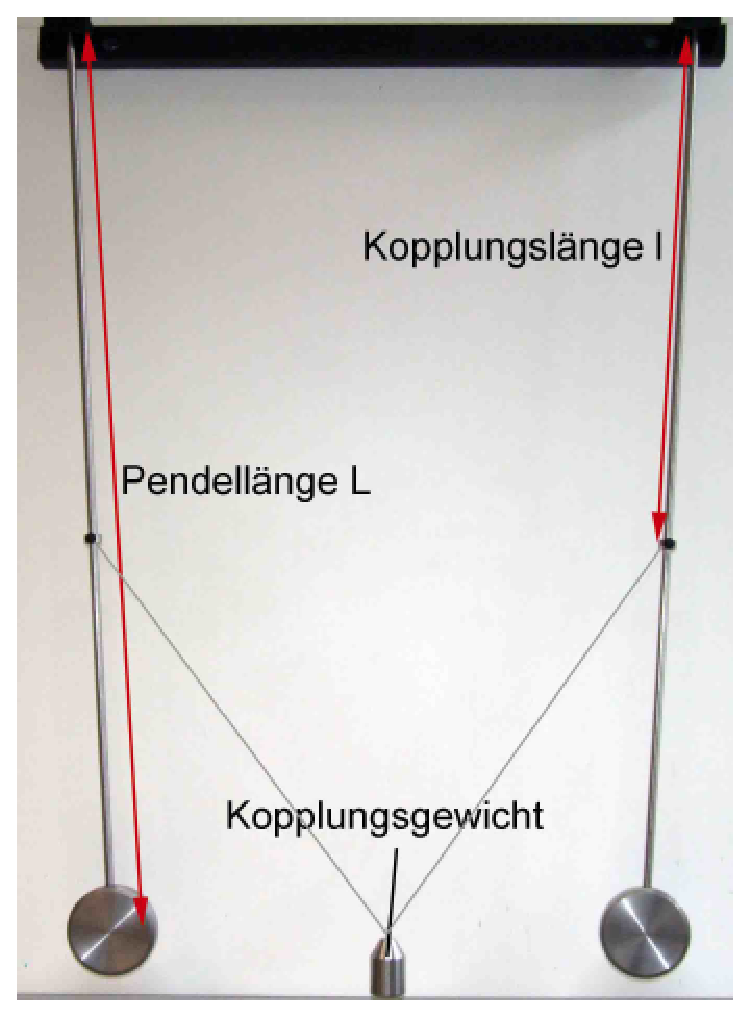
\includegraphics[width=0.9\linewidth]{gekoppelt.eps}
\end{subfigure}
\begin{subfigure}{0.6\textwidth}
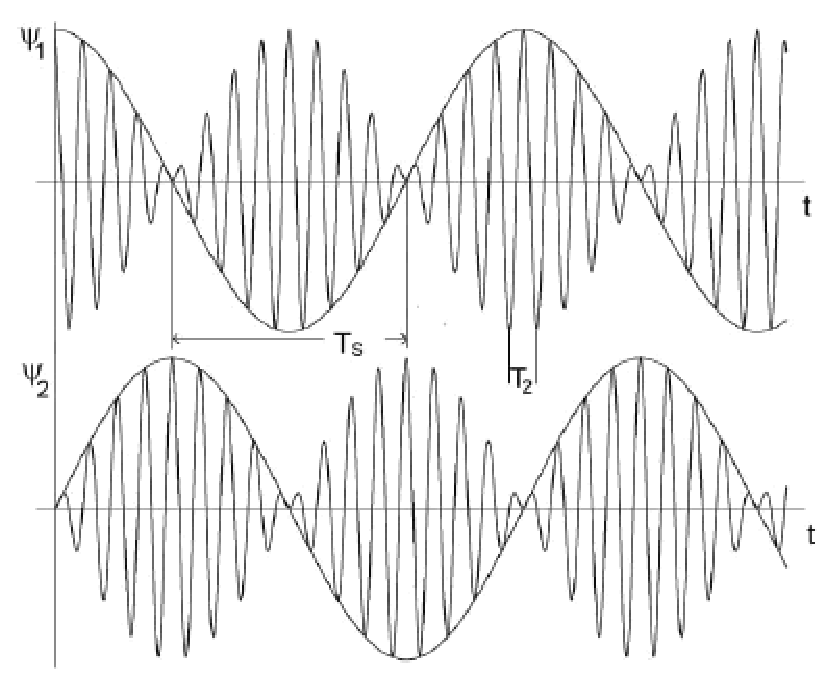
\includegraphics[width=0.9\linewidth]{schwebung.eps}
\end{subfigure}
\caption{\textit{Links:} Gekoppelte Pendel mit Kopplungslänge $l$, Pendellänge $L$ und Kopplungsgewicht $G$. \textit{Rechts:} Schwebung gekoppelter Pendel.}
\end{figure}

Beim gekoppelten Pendel gibt es drei Fälle zu unterscheiden:\\
Die \textbf{gleichsinnige Schwingung}, falls beide Pendel gleichzeitig in die gleiche Richtung angestoßen werden.\\
Die \textbf{gegensinnige Schwingung}, falls beide Pendel gleichzeitig in entgegengesetzter Richtung angestoßen werden.\\
Der \textbf{Schwebungsfall}, falls nur ein Pendel angestoßen wird, während sich das andere in Ruhe befindet.\\
\\
Für den Schwebungsfall sind die Frequenzen:
$$\omega_S=\frac{\omega_1 - \omega_0}{2}$$
$$\omega_S=\frac{\omega_1 + \omega_0}{2}$$
wo $\omega_0=\sqrt{D/J}$ und $\omega_1=\sqrt{(D+2D*)/J}$ mit dem Richtmoment aufgrund der Schwerkraft $D$, dem Richtmoment aufgrund der Kopplung $D*$ und dem Trägheitsmoment $J$.\\
\\
Der Kopplungsgrad kann dann durch die Eigenfrequenzen oder aus den Frequenzen der Schwebung berechnet werden:
$$K_{eigen}=\frac{\omega_1^2-\omega_0^2}{\omega_1^2+\omega_0^2}=$$
$$K_{schwebung}=\frac{2\omega_S \omega_2}{\omega_S^2 + \omega_2^2}$$
\\
Die Schwebungsdauer $T_S$ zwischen zwei Stillständen ist:
$$T_S=\pi/\omega_S$$

\subsection{Dopplerverschiebung}


\section{Aufbau}
\section{Messergebnisse}

\subsection{Drehpendel}
%Bestimmen Sie die Eigenfrequenz $\omega_0$ des Pendels.
Die Eigenfrequenz des Pendels:
$$\omega_0=\sqrt{\frac{D}{m}}=$$
\\
%Bestimmen Sie die Dämpfungskonstante $\delta$ und das zugehörige logarithmische Dekrement $\Lambda$.
Die Dämpfungskonstante ist
$$\delta_1=k/2m=$$
\\
Mit \ref{dekrement} Können wir das logarithmische Dämpfungsdekrement $\Lambda$ bestimmen:
$$\Lambda=ln\frac{x(nT)}{x((n+1)T)}=\delta T=$$
\\
%Nehmen Sie die Amplitudenresonanzkurve für einen Erregerfrequenzbereich $0.2-0.9\si{Hz}$ auf.
Die Erregerfrequenz des Motors:
$$\omega=$$
\\
Die Amplitudenresonanzkurve:
$$A^2=\frac{F_0^2}{m^2(\omega_0^2-\omega^2)^2+k^2\omega^2}=$$
\\
%Bestimmen Sie die Dämpfungskonstante $\delta$ aus der Halbwertsbreite der Resonanzkurve und vergleichen Sie das Ergebnis mit dem von Aufgabe 2.
Die Halbwertsbreite:
$$\Delta \omega=$$
\\
Die Dämpfungskonstante $\delta$ bestimmt aus der Halbwertsbreite der Resonanzkurve:
$$\delta_2=\frac{\Delta \omega}{2}=$$
\\
%Bestimmen sie Q für beide Dämpfungen und vergleichen Sie die Werte.
Der Gütefaktor $Q$:
$$Q=\omega_0/2\delta=\omega_0/\Delta \omega=$$

Gleichstrommessungenauigkeit: 2,5\% vom Skalenendwert (500mA)\\
$(100\pm 10) \si{mA}$

SChwingungsdauer:\\
$T_1=(1.83 \pm 0.01)\si{s}$
Eigenfrequenz $\omega_0$:\\
$\omega_0=(3.43 \pm 0.01)$

$\delta_1=-1.02 \pm 0.18$
Messung 2
$(150\pm10) \si{mA}$
SChwingungsdauer:\\
$T_2=(1.82 \pm 0.01)\si{s}$

$\delta_2= -0.0429 \pm 0.0038$

Erregerfrequenz 1: 0.8417 Hz

\subsection{Gekoppelte Pendel}

%Erfragen Sie zwei verschiedene Gewichte G und eine Kopplungslänge l vom Betreuer.
$$G_1=$$
$$G_2=$$
$$l=$$
\\
Wir stellen die geforderte Kopplungslänge $l$ ein:\\
Wir messen die Pendellänge $L$:
$$L=$$
\\
%Untersuchen Sie für jedes Gewicht die gleichsinnige und gegensinnige Schwingung sowie den Schwebungsfall.

%Berechnen Sie den Kopplungsgrad K aus den Eigenfrequenzen sowie aus den Frequenzen der Schwebung.
$$K_{eigen}=\frac{\omega_1^2-\omega_0^2}{\omega_1^2+\omega_0^2}=$$
$$K_{schwebung}=\frac{2\omega_S \omega_2}{\omega_S^2 + \omega_2^2}$$

\subsection{Dopplerverschiebung}


\section{Diskussion}
\subsection*{Drehpendel}
%Bestimmen Sie die Dämpfungskonstante $\delta$ aus der Halbwertsbreite der Resonanzkurve und vergleichen Sie das Ergebnis mit dem von Aufgabe 2.
%Bestimmen sie Q für beide Dämpfungen und vergleichen Sie die Werte.
\textbf{Dämpfungskonstante:}\\
$\delta_1=$, $\delta_2=$

\subsection*{Gekoppelte Pendel}
%Vergleichen und diskutieren Sie die Ergebnisse für die gewonnenen Kopplungsgrade.
\textbf{Kopplungsgrade:}\\
$K_{eigen}=$, $K_{schwebung}=$
\subsection*{Dopplerverschiebung}

%Bestimmen Sie die Grundfrequenz $\nu_0$ genau.

%Bestimmen Sie anschließend für jeweils 5 Wagengeschwindigkeiten +v bzw. -v (1-6 $\si{cm.s^{-1}}$) die Schwebungsdauern $T_S$.

% Benutzen Sie die Schwebungsdauern $T_S$ und Ihr Wissen aus Gekoppelte Pendel um die Schallgeschwindigkeit in Luft zu bestimmen.


\end{document}
